\chapter{有向图模型}
\label{chap:pgm-directed}

设备报警可以为故障提供线索，传感器失灵却也可以解释同一条报警。若随后确认传感器已经失灵，故障的后验概率就可能下降。同样是增加观测，给定过热状态可以屏蔽故障与报警之间的一条联系，给定报警状态却可能让两种解释产生关联。这些变化取决于观测节点在路径上的位置，有向图为判断它们提供了规则。

第~\ref{chap:pgm-overview}章用设备模型建立了“局部依赖组织联合分布”的整体印象：图上的箭头对应局部条件分布，把几个小概率表相乘就得到完整的联合分布。本章要把这一印象变成可以核对、可以证明的数学对象。具体要回答三件事：图上的箭头究竟对应怎样的独立性假设；给定部分观测后，图怎样判断哪些变量会独立；以及局部概率表怎样组合成可计算、可估计、可采样的模型。为此，本章先用一个固定变量顺序写出独立性假设，再用几种基本路径比较观测的作用，随后考察节点邻域及连接两组节点的全部路径。在此基础上，将这些关系与局部条件分布的乘积联系起来，并用离散表和连续条件分布给出可计算的模型。全局性质蕴含局部性质的图论证明随命题给出，其余跨表示证明集中在第~\ref{sec:pgm-representations-directed-proofs}节；这些结论共同说明独立性语义、联合分解和数值参数化怎样配合。

\section{有向图模型的定义}
\label{sec:pgm-directed-definition}

用四个二值随机变量表示设备状态：故障$F$、过热$H$、报警$A$和传感器失灵$S$，取值$1$表示相应状态出现。图~\ref{fig:pgm-directed-device}采用$F\to H\to A\leftarrow S$三条箭头，对应如下局部假设：过热的条件分布以故障为输入，报警的条件分布以过热和传感器状态为输入。这个结构是用于说明概率语义的人工模型，后文的数值例子也采用教学参数。

\begin{figure}[htbp]
  \centering
  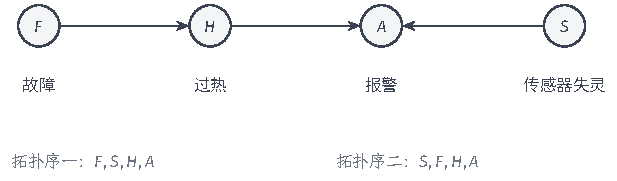
\includegraphics[width=104.482mm]{figures/09-probabilistic-graphical-models/01-representation/tikz/pgm-directed-device/figure.pdf}
  \caption{设备诊断的有向图及两个拓扑序。箭头指定局部条件分布的输入，$F$与$S$是没有父节点的根节点。下方两个序列都把父节点排在子节点之前，对应同一个图结构。}
  \label{fig:pgm-directed-device}
\end{figure}

把图写成$\mathcal G=(V,E)$，其中节点对应随机变量，箭头对应节点之间可能存在的直接依赖。本部分采用有限有向无环图，并排除自环；其他结构将在使用处另行说明。图的表示、拓扑排序及后文所用的路径分离规则，可参考\BookPartRef{part:graphs}{卷1《数学准备：计算、分析与几何》的“图”部分}。

箭头进入一个节点，说明该节点的局部条件分布要使用这个输入；但后续的独立性判断还需要反复引用另外两类关系：谁沿着箭头能“直接到达”谁，以及谁沿着箭头能“间接到达”谁。为了不再每次重新描述这些关系，先给它们命名。局部条件分布所用的直接输入，在图中组成节点$i$的\term{父节点}（parent）集合$\operatorname{pa}(i)$；$i$直接指向的节点组成\term{子节点}（child）集合$\operatorname{ch}(i)$。将直接连接扩展为长度至少为一的有向路径，能够到达$i$的节点组成\term{祖先}（ancestor）集合$\operatorname{an}(i)$，从$i$能够到达的节点组成\term{后代}（descendant）集合$\operatorname{de}(i)$，两者都排除$i$自身。在设备图中，$\operatorname{pa}(A)=\{H,S\}$、$\operatorname{an}(A)=\{F,H,S\}$，而$\operatorname{de}(S)=\{A\}$。这些例子用变量名标记节点，一般公式则用$A\subseteq V$表示节点集合、用$\bm{X}_A$表示相应随机向量。

后文会按某个顺序把各个节点的条件分布依次写出来，因此还需要一个“谁先谁后”的约定。按顺序指定条件分布时，父节点必须先于子节点出现；否则写子节点的条件分布时，父节点的取值还没有定义。有限有向无环图总能找到这样的顺序，称为拓扑序（topological order），而且可能有多个；图~\ref{fig:pgm-directed-device}中的$F,S,H,A$和$S,F,H,A$便是两个例子。两个合法拓扑序都满足同一规则：每条箭头从较前的位置指向较后的位置。

固定其中一个拓扑序，并将节点按该序重标记为$1,\ldots,d$。在处理节点$i$时，已经出现的节点组成\term{前驱集合}（predecessor set）$\operatorname{pre}(i)=\{1,\ldots,i-1\}$。前驱集合是顺序概念，父节点集合是图概念，两者并不相同：父节点属于前驱集合，因为父节点一定排得比子节点早；其他前驱则可能只是排在前面，例如互不相连的两个节点仍有先后次序。因此，当前顺序提供的全部条件与局部分布实际采用的父节点条件，需要分别记录——前驱中有一部分是“多余的”，图要说明的正是它们可以被省去。

\begin{definition}[有序Markov假设与有向图模型]
  \label{def:pgm-directed-ordered}
  给定有向图$\mathcal{G}$及一个固定拓扑序，若联合分布$p$对每个$i\in V$满足
  \begin{equation}
    X_i\perp
    \bm{X}_{\operatorname{pre}(i)\setminus\operatorname{pa}(i)}
    \mid\bm{X}_{\operatorname{pa}(i)},
    \label{eq:pgm-directed-ordered}
  \end{equation}
  则称它满足该顺序下的\term{有序Markov假设}（ordered Markov assumption）。\term{有向图模型}（directed graphical model）是有向图及其节点随机变量的联合分布，其中该联合分布满足上述假设。文献中传统上也称这类模型为\term{贝叶斯网络}（Bayesian network）；本书统一使用“有向图模型”。
\end{definition}

式~\eqref{eq:pgm-directed-ordered}把按顺序排在$X_i$前面的节点分成两组：父节点作为已知条件，其余前驱与$X_i$独立。直白地说，假设要求“当父节点的取值已经知道时，排在更前面的其他节点不再提供关于$X_i$的新信息”。这里约束的是整个分布，而均值或相关系数只描述它的部分特征。父集为空的根节点省去条件，前驱也为空时则没有需要约束的其他变量。

设备顺序$F,S,H,A$中的非平凡假设写为
\[
  S\perp F,\qquad H\perp S\mid F,\qquad A\perp F\mid(H,S).
\]
三个陈述可以逐条读出图的含义：$S\perp F$说两个根节点彼此独立；$H\perp S\mid F$说给定故障状态后，传感器失灵不再改变过热的概率；$A\perp F\mid(H,S)$说给定过热与传感器状态后，故障不再提供关于报警的额外信息。这些假设当前针对选定的顺序。后面的因子分解等价关系将说明，由一个拓扑序得到的模型也满足其他合法拓扑序下的有序性质，因此所定义的模型类与具体拓扑序无关。完整证明见第~\ref{sec:pgm-representations-directed-proofs}节。

$p$表示相对于坐标参考测度乘积的联合质量或密度，条件分布等式按条件变量的分布几乎处处成立。后文用有限离散求和展示计算，密度情形在相应条件下采用积分，有向模型的结论允许联合分布取零值。离散质量以计数测度求和，通常的连续密度以Lebesgue测度积分，二者都用完整条件分布而非单个矩描述独立性；相关概率工具可参考\BookChapterRef{chap:random-variables}{卷2《数学准备：概率、因果与决策》的“随机变量与概率基础”章}。对首次阅读可以这样理解：离散情形中上述等式就是按概率求和逐点成立，连续情形中是密度函数的等式，在零概率或零密度的配置上不必细究。

有向边为局部条件分布指定可用的输入，具体参数决定该输入是否实际改变输出分布。用$F$预测$H$描述的是观测条件下的分布，主动改变$F$后的结果则需要干预语义。第~\ref{chap:pgm-structure-learning}章将讨论赋予有向结构因果解释所需的假设与识别条件。

\Needspace{6\baselineskip}
\section{两个变量之间的四种基本关系}
\label{sec:pgm-directed-motifs}

第~\ref{sec:pgm-directed-definition}节把箭头解释成局部条件分布的输入，但要判断给定观测后两个变量是否独立，还需要知道信息沿箭头怎样流动。一条连接路径上的中间节点有不同的箭头形状，观测对它们的作用也不同：给定某些中间节点会“截断”两端的联系，给定另一些中间节点反而会“接通”两端。图~\ref{fig:pgm-directed-motifs}从直接连接、链、分叉和碰撞四种关系说明这种差别。下述三节点结论采用只有图中所画边的小图，描述结构对所有相容分布保证的独立性。在更大的图中，同样的判断用于逐条路径，最终还需检查其他连接路径；一条路径活跃时，实际依赖由具体参数决定。

\begin{figure}[htbp]
  \centering
  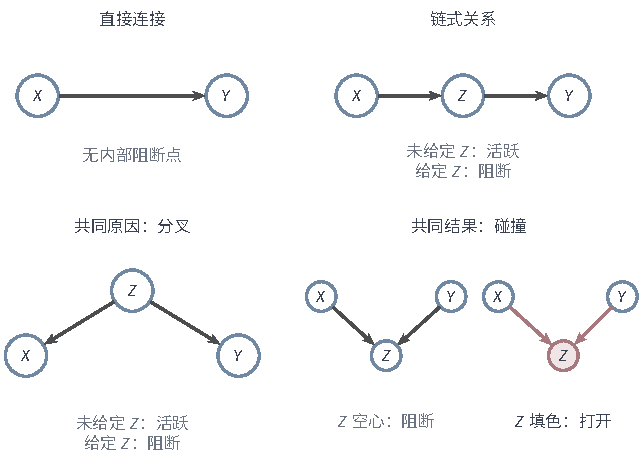
\includegraphics[width=108.793mm]{figures/09-probabilistic-graphical-models/01-representation/tikz/pgm-directed-motifs/figure.pdf}
  \caption{四种局部关系及观测中间节点后的路径变化。链和分叉在同一小图中对照两种状态；碰撞关系分为两列，空心$Z$表示未观测的阻断点，红色填充$Z$表示给定后打开的位置。活跃路径允许两端存在依赖，具体参数决定依赖是否出现。在大图中，观测碰撞点的后代也会打开该位置；直接连接没有内部阻断点。}
  \label{fig:pgm-directed-motifs}
\end{figure}

\paragraph{直接连接}
在直接连接$X\to Y$中，$X$进入$Y$的局部分布，路径中没有可用于阻断的中间节点：$Y$的条件分布直接以$X$为输入，中间没有任何变量可以“接住”这条信息。路径判断因此没有内部位置可以给定。需要提醒的是，结构允许依赖不等于实际一定有依赖：具体条件表若满足$p(y\mid x)=p(y)$，这个输入仍可能不改变分布，即该参数下$X\perp Y$。第~\ref{sec:pgm-directed-sound-complete}节将用数值例子说明结构允许的依赖与单个分布实际具有的依赖之间的区别。

\paragraph{链}
链式关系$X\to Z\to Y$让信息先传到中间的$Z$，再传到$Y$。这里的$Z$像是两端之间的“中介”：关于$X$的信息只有通过$Z$才能影响$Y$，因此一旦$Z$的取值已知，$X$就不再提供关于$Y$的新信息。采用顺序$X,Z,Y$，有序假设给出$Y\perp X\mid Z$，对应乘积$p(x,z,y)=p(x)p(z\mid x)p(y\mid z)$，一般等价证明见第~\ref{sec:pgm-representations-directed-proofs}节。给定一个满足$p(z)>0$的中间状态，条件联合分布为
\[
  p(x,y\mid z)=p(x\mid z)p(y\mid z).
\]
消去$Z$时，各个$z$下的条件分布混合在一起，两端通常仍有关联。一个具体数值例子可以说明这种“给定后独立、不给定则相关”的差别。设$X$等概率取$0,1$，$Z$依赖$X$：$p(Z=1\mid X=1)=0.8$、$p(Z=1\mid X=0)=0.2$，$Y$再依赖$Z$：$p(Y=1\mid Z=1)=0.9$、$p(Y=1\mid Z=0)=0.1$。于是$p(Z=1)=0.5\times0.8+0.5\times0.2=0.5$，$p(Y=1)=0.5\times0.9+0.5\times0.1=0.5$；两端联合出现的概率为
\[\begin{aligned}
  p(X=1,Y=1)
  &=\sum_z p(X=1)\,p(Z=z\mid X=1)\,p(Y=1\mid Z=z)\\
  &=0.5\times(0.8\times0.9+0.2\times0.1)=0.37,
\end{aligned}\]
大于$p(X=1)p(Y=1)=0.5\times0.5=0.25$，说明不知道$Z$时两端相关。而给定$Z=1$后，
\[
  p(X=1\mid Z=1)
  =\frac{0.5\times0.8}{0.5}=0.8,\qquad
  p(Y=1\mid Z=1)=0.9,
\]
条件联合
\[
  p(X=1,Y=1\mid Z=1)
  =\frac{0.5\times0.8\times0.9}{0.5}=0.72,
\]
正好等于两者乘积。两端的相关完全由中间变量$Z$造成，给定$Z$后独立。将链反向画成$X\leftarrow Z\leftarrow Y$，给定中间节点后的独立关系相同。因此，路径判断考察内部节点的箭头形状，而非从某一端是否能沿箭头走到另一端。

\paragraph{分叉}
分叉$X\leftarrow Z\to Y$以同一节点作为两端的条件，常用“共同原因”辨认其形状：两端的共同变化来自同一个源头$Z$，固定$Z$后，两端各自剩余的随机变化没有共享来源，于是独立；不知道$Z$时，两端的共同变化使它们相关。给定$Z$时，图保证$X\perp Y\mid Z$；消去$Z$后，混合分布则可能相关。设$Z$等概率取$0$或$1$，给定$Z$后$X,Y$独立，并且两者取$1$的概率在$Z=1$时均为$0.9$，在$Z=0$时均为$0.1$。此时$p(X=1)=p(Y=1)=0.5$，而$p(X=1,Y=1)=(0.9^2+0.1^2)/2=0.41\ne0.25$。这个差值来自不同$Z$状态的混合，与每个固定$Z$下的条件独立相容：$X$与$Y$并不直接相互影响，它们只是随$Z$一起变动。

\paragraph{碰撞}
碰撞结构$X\to Z\leftarrow Y$将两条箭头的终点放在同一个中间节点，也称“共同结果”结构。两个根节点独立，联合分解为$p(x)p(y)p(z\mid x,y)$，对$z$求和后得到$p(x,y)=p(x)p(y)$，所以不观测$Z$时两端保持独立。给定$z$时，局部因子$p(z\mid x,y)$参与条件概率，可能使两端产生依赖：一旦知道共同结果已经发生，两端就会竞争对这个结果的解释。设$X,Y$是独立公平二值变量，$Z=1$当且仅当至少一个输入为$1$；给定$Z=1$时，$p(X=1\mid Z=1)=2/3$，再给定$Y=1$时则降为$1/2$。在这个参数设定中，确认$Y$已能解释共同结果，就降低了$X$取$1$的条件概率。这称为\term{解释消除}（explaining away），即观测共同结果后，不同解释之间产生竞争。具体依赖的方向和强弱仍由条件概率决定。

\paragraph{碰撞点的后代}
观测碰撞点的后代也可能提供关于碰撞点的信息，因此路径判据将这个位置视为打开。例如，在$X\to Z\leftarrow Y$后接$Z\to D$，若$D=Z$，观测$D$便等价于观测$Z$；若$D$是带噪声的测量，则传递的信息量取决于噪声水平。碰撞点及全部后代均未给定时，该位置才由图保证阻断。这里的“共同原因”和“共同结果”描述箭头形状，其因果解释需要另行建立。

为把“碰撞点自身或后代被给定”写成集合条件，先用$T$表示被给定节点的集合，并记
\[
  \operatorname{an}^{+}(T)
    =T\cup\bigcup_{t\in T}\operatorname{an}(t).
\]
这个祖先闭包包含$T$自身和$T$中各节点的全部祖先。节点$Z$属于该集合，表示$Z$自身被给定，或者它有被给定的后代。图~\ref{fig:pgm-directed-collider-descendant}用$S$表示条件节点集合，右图中$S=\{D\}$；这里的集合记号$S$与设备例子中的传感器变量$S$由上下文区分。因此右图的$Z\in\operatorname{an}^{+}(S)$正是在说$Z$是已观测节点$D$的祖先。

\begin{figure}[htbp]
  \centering
  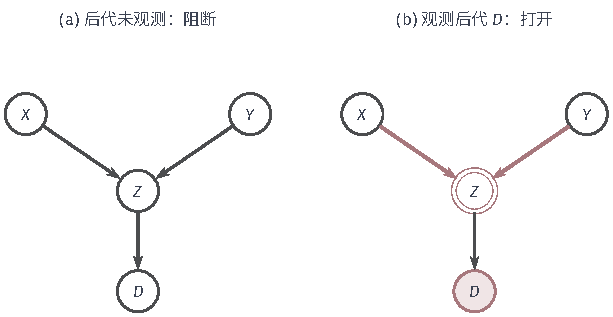
\includegraphics[width=103.720mm]{figures/09-probabilistic-graphical-models/01-representation/tikz/pgm-directed-collider-descendant/figure.pdf}
  \caption{后代观测对碰撞位置的作用。左图中$Z$及其后代均未给定，路径$X\to Z\leftarrow Y$被阻断；右图将后代$D$填色为观测，空心双圈$Z$标出已打开的碰撞位置，红色路径满足$Z\in\operatorname{an}^{+}(S)$。图上打开的路径允许依赖出现，依赖强度由分布决定。}
  \label{fig:pgm-directed-collider-descendant}
\end{figure}

\section{有向图的局部独立性}
\label{sec:pgm-directed-local}

第~\ref{sec:pgm-directed-definition}节的有序Markov假设依赖于一个固定拓扑序：给定父节点后，排在前面的其他节点不再提供信息。图给出的独立性不应依赖于所选排列顺序。给定父节点以后，可以从$X_i$的条件中省去全部非后代节点；前驱集合只能回答一个固定顺序内的问题，非后代集合则不依赖排列。将节点自身与全部后代排除，记为
\[
  \operatorname{nd}(i)=V\setminus\bigl(\{i\}\cup\operatorname{de}(i)\bigr).
\]
之所以要排除后代，是因为后代受$X_i$影响、携带关于$X_i$的信息：即使父节点已知，子节点仍然可能反映当前节点的状态。父节点属于这个集合，因为父节点若同时是后代，就会与指向$i$的边组成有向环。集合排除$i$自身，随后还要把已经作为条件的父节点从待独立的变量中分出。

\begin{definition}[局部Markov性质]
  \label{def:pgm-directed-local-markov}
  分布$p$满足有向图$\mathcal{G}$的\term{局部Markov性质}（local Markov property），是指对每个节点$i$，
  \begin{equation}
    X_i\perp
    \bm{X}_{\operatorname{nd}(i)\setminus\operatorname{pa}(i)}
    \mid\bm{X}_{\operatorname{pa}(i)}.
    \label{eq:pgm-directed-local-markov}
  \end{equation}
\end{definition}

局部Markov性质用父节点屏蔽其他非后代：给定父节点后，既非父节点又非后代的节点不再改变$X_i$的条件分布。后代仍可能反映当前节点的状态，例如在设备模型中给定$F$以后，报警$A$还可以为过热$H$提供观测线索。因此，式~\eqref{eq:pgm-directed-local-markov}限定独立对象为非父、非后代节点。

合法拓扑序中的前驱都属于非后代，局部性质因而可以通过边缘化无须保留的独立变量，得到有序性质。相反方向涉及更多节点：在$F,S,H,A$顺序中，有序性质给出$S\perp F$，局部性质还包括排在$S$后面的$H$，即$S\perp(F,H)$。这一步需要联合分布的因子分解与祖先边缘化，证明见第~\ref{sec:pgm-representations-directed-proofs}节。两方向并不对称：局部性质包含更多的独立陈述，强于固定顺序下的有序性质。

若查询要求在给定一组变量后，使$X_i$与这组之外的其他变量独立，就还要处理后代所携带的信息。能完成这种屏蔽的一组变量称为\term{Markov毯}（Markov blanket）。我们先看哪些信息必须由这组变量接住，再写出一般集合。

在设备模型中，给定故障$F$仍不能忽略报警$A$，因为$A$可以提供过热$H$的线索，所以屏蔽集合还要纳入子节点$A$。但报警也可能由传感器失灵$S$解释：已经知道$A=1$时，再得知$S$的状态，可能改变我们对$H$的判断。因此只把父节点和子节点纳入条件还不够，子节点的其他父节点$S$也要纳入。这里出现的是$H\to A\leftarrow S$的形状，两条箭头在共同子节点$A$处相遇；给定共同结果可能使其两端的解释产生联系。第~\ref{sec:pgm-directed-motifs}节已将这种相遇称为碰撞，并用共同结果及其后代的观测说明路径怎样打开；这里把该机制用于确定屏蔽集合。

在一般图中，同样要处理$X_i\to C\leftarrow U$这样的首段。给定子节点$C$后，$U$仍可能改变对$X_i$的判断；若$U$还连接其他节点，这些节点的信息也可能沿此首段传来。将$U$一起给定，便可屏蔽从$U$继续通向集合外的联系。把父节点、子节点及每个子节点的其余父节点合并，有向图为节点$i$提供如下标准集合：
\begin{equation}
  \begin{aligned}
    \operatorname{mb}(i)
    ={}&\operatorname{pa}(i)\cup\operatorname{ch}(i)\\
       &{}\cup\bigcup_{j\in\operatorname{ch}(i)}
           \bigl(\operatorname{pa}(j)\setminus\{i\}\bigr).
  \end{aligned}
  \label{eq:pgm-directed-blanket}
\end{equation}
该集合同时包含父节点、子节点和子节点的其他父节点，图~\ref{fig:pgm-directed-markov-blanket}分别以$P,C,U$标示。标准集合将子节点纳入条件，以处理它们对$X_i$提供的线索；给定子节点还会打开在该处碰撞的路径，于是集合同时纳入其余父节点。给定完整集合后，毯外节点$O$与$X_i$之间的路径得到屏蔽，即使$O$在原图中与毯内变量相连。

\begin{figure}[htbp]
  \centering
  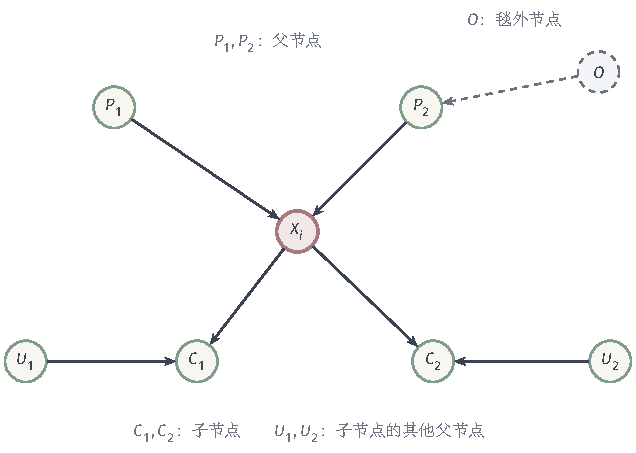
\includegraphics[width=107.685mm]{figures/09-probabilistic-graphical-models/01-representation/tikz/pgm-directed-markov-blanket/figure.pdf}
  \caption{节点$X_i$的图上Markov毯。父节点$P_1,P_2$、子节点$C_1,C_2$以及子节点的其他父节点$U_1,U_2$共同组成$\operatorname{mb}(i)$；以虚线描边的$O$位于毯外。}
  \label{fig:pgm-directed-markov-blanket}
\end{figure}

\begin{theorem}[有向图中的Markov毯]
  \label{thm:pgm-directed-markov-blanket}
  设$\mathcal{G}=(V,E)$为有限有向无环图，$p$为节点随机变量$\bm{X}=(X_i)_{i\in V}$的联合分布，且$(\mathcal{G},p)$构成有向图模型。则对每个节点$i\in V$，
  \[
    X_i\perp
    \bm{X}_{V\setminus(\{i\}\cup\operatorname{mb}(i))}
    \mid\bm{X}_{\operatorname{mb}(i)}.
  \]
\end{theorem}

在设备模型中，$\operatorname{mb}(H)=\{F,A,S\}$，其中$S$作为子节点$A$的另一个父节点进入毯。式~\eqref{eq:pgm-directed-blanket}由结构保证屏蔽关系，特定参数若产生冗余，则还可能使用更小的集合。定理~\ref{thm:pgm-directed-markov-blanket}的证明见第~\ref{sec:pgm-representations-directed-proofs}节。

\section{有向图的全局独立性}
\label{sec:pgm-directed-global}

报警状态给定后，故障与传感器失灵是否独立，涉及两个节点之间的整条路径，而不只是单个局部位置。第~\ref{sec:pgm-directed-motifs}节的四种基本关系只回答了“单条路径上的一个内部节点”怎样影响两端；实际问题中，两组节点之间往往存在多条路径，给定条件会同时作用于所有路径。全局Markov性质将查询扩展为任意两组节点，由所有连接路径共同判断独立性。本节将第~\ref{sec:pgm-directed-motifs}节的基本路径规则汇总为所有连接路径的判据，再证明全局性质能够推出局部性质和固定拓扑序下的有序性质；第~\ref{sec:pgm-directed-ci-to-factor}节将把它们与因子分解联系起来。

\subsection{d-分离的定义}
\label{sec:pgm-directed-d-separation}

两组节点在给定条件后仍可能通过多条路径联系，因而分离查询需要汇总全部路径的判断。单条路径是否活跃，由其中每个内部位置共同决定：路径上的非碰撞点被给定时阻断路径，碰撞点自身或后代被给定时则打开该位置。整条路径活跃，要求每个内部位置都满足自己的条件；一个位置的打开无法消除另一位置的阻断。对两两不交的$A,B,S\subseteq V$，若$A,B$之间不存在活跃路径，就记$A\perp_{\mathcal G}B\mid S$。这个记号先描述图上的分离，随后将说明它与概率独立的关系。这里继续沿用包含集合自身的祖先闭包$\operatorname{an}^{+}(T)$，用它记录哪些碰撞点具有自身或后代的观测证据。

设备路径中的$A$是碰撞点，$H$是非碰撞点，图~\ref{fig:pgm-directed-active-path}对照了给定它们后的变化。只给定$A$时路径活跃，再给定$H$时路径在$H$处阻断。整条路径活跃需要每个内部位置都满足条件，因此一个位置的打开无法消除另一位置的阻断。

\begin{figure}[htbp]
  \centering
  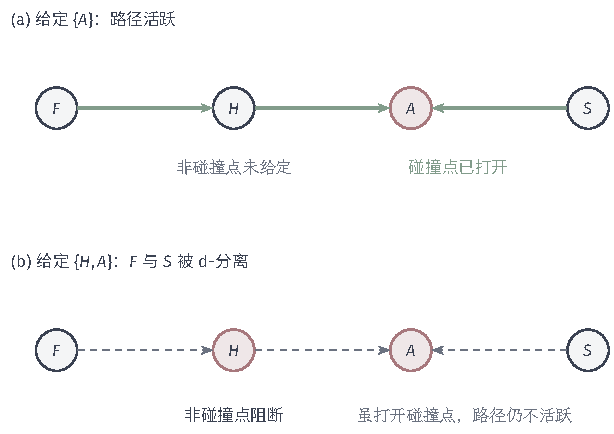
\includegraphics[width=103.904mm]{figures/09-probabilistic-graphical-models/01-representation/tikz/pgm-directed-active-path/figure.pdf}
  \caption{设备路径的活跃状态与d-分离。上图给定碰撞点$A$后，$F\to H\to A\leftarrow S$活跃；下图再给定非碰撞点$H$后，唯一的连接路径被阻断，得到$F\perp_{\mathcal{G}}S\mid(H,A)$。红色节点为给定变量，绿色实线为活跃路径，灰色虚线为阻断路径。}
  \label{fig:pgm-directed-active-path}
\end{figure}

图上的$A\perp_{\mathcal G}B\mid S$与分布中的$\bm{X}_A\perp\bm{X}_B\mid\bm{X}_S$分别描述路径和概率关系：前者是图的分离查询，后者是分布的条件独立。\term{全局Markov性质}（global Markov property）把两者接起来：对每个两两不交的查询$(A,B,S)$，图中的d-分离蕴含相应的分布独立。第~\ref{sec:pgm-directed-sound-complete}节将说明相容分布为何满足这个蕴含。

\begin{lemma}[全局Markov性质蕴含局部Markov性质]
  \label{lem:pgm-representations-global-to-local}
  设$\mathcal{G}=(V,E)$为有限有向无环图，$p$为节点随机变量$\bm{X}=(X_i)_{i\in V}$的联合分布。若$p$满足$\mathcal{G}$的全局Markov性质，则$p$也满足该图的局部Markov性质，并进一步满足任一固定拓扑序下的有序Markov性质。
\end{lemma}

\begin{proof}[引理~\ref{lem:pgm-representations-global-to-local}的证明]
证明的思路是固定一个节点$i$，逐一考察它到每个非父、非后代节点的路径，说明给定父集$\operatorname{pa}(i)$后，每条这样的路径都会在某处被阻断。固定节点$i$，逐一考察它到非父、非后代节点的路径。路径若在$i$处经过一条入边，邻接的父节点就是内部非碰撞点，给定$\operatorname{pa}(i)$即可在此阻断。路径若先沿$i$的出边前进，则到达非后代之前必须改变沿箭头前进的方向；第一次转折的首段形如$i\to v_1\to\cdots\to v_k\leftarrow v_{k+1}$，所以$v_k$是碰撞点，也是$i$的后代。转折前一直顺箭头前进；若直到终点都没有转折，终点本身就会是$i$的后代，与所考察端点的范围矛盾。这个碰撞点及其后代均在父集之外：若其中某点$u$属于父集，就存在从$i$经过$v_k$到$u$的有向路径，再接$u\to i$构成有向环。因此给定父集不会观测该碰撞点或其后代，它仍保持阻断。两类路径都被阻断，得到
\[
  i\perp_{\mathcal G}
  \operatorname{nd}(i)\setminus\operatorname{pa}(i)
  \mid\operatorname{pa}(i).
\]
将该图分离代入全局Markov性质，便得到局部Markov性质。合法拓扑序的前驱包含于非后代集合，从局部独立陈述中边缘化其他非后代，又得到该拓扑序下的有序Markov性质。
\end{proof}

在设备图中，$F,S$只有$F\to H\to A\leftarrow S$这一条连接路径。无观测时，碰撞点$A$阻断它，得到$F\perp S$；给定报警$A$后，碰撞位置打开而$H$保持未观测，路径转为活跃；再给定$H$后又得到$F\perp S\mid(H,A)$。如果增加$A\to D$，观测$D$同样会打开$A$，因为它提供了碰撞点后代的证据。

条件集合$S$记录被给定的变量，而具体取值另行指定。d-分离所对应的条件独立对条件变量分布几乎处处成立，涵盖整项条件关系。某些参数还可能只在特定条件取值下产生独立，这类上下文性质来自具体分布，须与图上的分离查询分别处理。

\subsection{d-分离的可靠性与特定场景下的完备性}
\label{sec:pgm-directed-sound-complete}

同一张图可以配上不同的条件概率表，路径判据因而需要在分布类上解释。这里需要区分两个方向相反的问题。分离查询应对所有相容分布成立：只要图分离，就不允许任何相容分布表现出依赖，这称为可靠性。未分离查询则相反，需要考察是否存在某个实际依赖的相容分布：图没有分离，并不保证每个分布都依赖，只要求“存在一个”相容分布依赖，这称为模型类完备性。记$\mathcal{M}(\mathcal{G})$为定义~\ref{def:pgm-directed-ordered}所给模型的分布类；第~\ref{sec:pgm-directed-factorization}节将说明它与按$\mathcal{G}$分解的分布类等价，证明见第~\ref{sec:pgm-representations-directed-proofs}节。

\begin{theorem}[d-分离的可靠性]
  \label{thm:pgm-directed-soundness}
  设$\mathcal{G}=(V,E)$为有限有向无环图，$A,B,S\subseteq V$两两不交且$A,B$非空。对每个$p\in\mathcal{M}(\mathcal{G})$，
  \begin{equation}
    A\perp_{\mathcal{G}}B\mid S
    \quad\Longrightarrow\quad
    \bm{X}_A\perp_p\bm{X}_B\mid\bm{X}_S.
    \label{eq:pgm-directed-soundness}
  \end{equation}
\end{theorem}

\begin{example}[未分离但独立的固定分布]
  \label{ex:pgm-directed-unseparated-independent}
  在只有一条边$X\to Y$的图中，令$X,Y\in\{0,1\}$，并设$p(X=0)=p(X=1)=1/2$。对每个$x\in\{0,1\}$，都取$p(Y=1\mid X=x)=1/3$和$p(Y=0\mid X=x)=2/3$。图上两个节点直接相邻，空集无法将它们d-分离；条件表的两行却相同，边缘化$X$得到$p(Y=1)=1/3$和$p(Y=0)=2/3$。由此对所有$x,y\in\{0,1\}$有
  \[
    p(X=x,Y=y)
    =
    p(X=x)p(Y=y)
    =
    \begin{cases}
      1/6,&y=1,\\
      1/3,&y=0.
    \end{cases}
  \]
  这个乘积等式给出该固定分布中的$X\perp Y$，说明相邻节点在某些参数下也能独立。图中保留这条边没有“错”，只是这个特定的参数选择没有让它发挥作用。
\end{example}

示例~\ref{ex:pgm-directed-unseparated-independent}区分了已选定的分布与可选的分布类。该分布中的依赖可以消失，而在充分丰富的分布类中，每项未分离查询仍有至少一个相容分布表现出依赖。后一种存在性结论称为\term{模型类完备性}，以下分别在严格正有限离散模型类与非退化线性高斯模型类中陈述。

\term{严格正有限离散模型}中，每个变量有有限个状态，每个完整配置的联合概率均大于$0$。固定状态空间$\mathcal{X}_i$并要求$|\mathcal{X}_i|\geq2$，将其中严格为正且按$\mathcal{G}$分解的质量函数记为$\mathcal{M}_{\mathrm{disc}}^{+}(\mathcal{G})$。要求概率严格为正，是为了让条件概率都能用比值计算：条件事件概率为零时，条件分布没有定义。\term{非退化线性高斯模型}则以父节点的线性函数加独立高斯噪声表示当前节点；正噪声方差保证联合分布具有完整维度。将所有由下式生成的分布记为$\mathcal{M}_{\mathrm{LG}}(\mathcal{G})$：
\[
  X_i=a_i+\sum_{j\in\operatorname{pa}(i)}b_{i,j}X_j+\varepsilon_i
\]
其中$a_i$是节点$i$的实值截距，即不随父节点取值改变的常数偏移；边系数$b_{i,j}$可取任意实数，描述父变量$X_j$对当前条件均值的线性贡献。噪声$\varepsilon_i$相互独立，满足$\varepsilon_i\sim\mathcal{N}(0,\sigma_i^2)$及$\sigma_i^2>0$。正方差保证每个节点都保留自己的随机变化：若某个方差为零，该节点退化为父节点的确定性函数，联合分布会塌缩到低维子空间。

\begin{theorem}[d-分离在特定模型类中的完备性]
  \label{thm:pgm-directed-completeness}
  设$\mathcal{G}=(V,E)$为有限有向无环图，$A,B,S\subseteq V$两两不交且$A,B$非空。若
  \[
    A\not\perp_{\mathcal{G}}B\mid S,
  \]
  则分别存在$p_{\mathrm{disc}}\in\mathcal{M}_{\mathrm{disc}}^{+}(\mathcal{G})$与$p_{\mathrm{LG}}\in\mathcal{M}_{\mathrm{LG}}(\mathcal{G})$，使
  \begin{equation}
    \bm{X}_A\not\perp_{p_{\mathrm{disc}}}\bm{X}_B\mid\bm{X}_S,
    \qquad
    \bm{X}_A\not\perp_{p_{\mathrm{LG}}}\bm{X}_B\mid\bm{X}_S.
    \label{eq:pgm-directed-completeness}
  \end{equation}
\end{theorem}

可靠性覆盖每个相容分布，模型类完备性则为每项未分离查询提供一个不独立的见证分布，不同查询还可以使用不同见证。两种结论采用不同量词，因此完备性与前面的固定分布反例相容：反例说“某一个分布”可以独立，完备性说“每一个未分离查询都存在另一个分布”表现出依赖。两个定理的证明见第~\ref{sec:pgm-representations-directed-proofs}节。

从观测到的条件独立反推图结构时，上例的相同行会造成歧义：独立可能来自缺边，也可能来自参数。这正是引入忠实性的原因。

对于$p\in\mathcal{M}(\mathcal{G})$，模型的Markov性已经使图分离推出概率独立。忠实性进一步要求，每项分布独立都能由图分离解释；观测独立与结构识别之间的关系，可参考\BookChapterRef{chap:causal-inference}{卷2《数学准备：概率、因果与决策》“因果响应”章}。两个方向共同成立时，图与分布的独立关系集合相同：图分离恰好对应分布独立，不多也不少。

确定性关系、强制参数共享和参数抵消都可能产生额外独立性。有向分解允许这些参数，而忠实性对分布施加进一步限制。结构学习在依据独立性删边时，需要说明所采用的忠实性假设及其适用依据。参数抵消可以理解为不同路径对同一变量的贡献相加后变为零。例如，若$X_2=2X_1+\varepsilon_2$、$X_3=-2X_1+X_2+\varepsilon_3$，且$X_1,\varepsilon_2,\varepsilon_3$相互独立，则代入后$X_3=\varepsilon_2+\varepsilon_3$，不再依赖$X_1$。直接路径与经过$X_2$的路径仍在图上，但它们对$X_3$中$X_1$系数的贡献$-2$与$2$恰好抵消。这只展示额外独立的一种参数情形，不表示所有共享参数或确定性关系都会破坏忠实性。

\subsection{d-分离的检测}
\label{sec:pgm-directed-d-separation-testing}

路径判据可直接用于小图：逐条路径检查内部节点即可。但大图中的许多不同路径会共享同一节点，并从相同方向到达该节点，逐条枚举路径的数量可能随图规模指数增长。检测算法可以合并这些路径的到达状态，也可以将当前查询转为无向图的连通性检查。下面分别说明这两种计算方式如何利用结构。

\begingroup
% tufte-book禁用subsubsection；本节局部沿用其支持的第三级paragraph样式。
\let\subsubsection\paragraph

\subsubsection{Bayes--ball算法}
\label{sec:pgm-directed-bayes-ball}

设备图对$F,S$的查询只有一条连接路径，可以按内部节点的角色逐项检查，结果列于表~\ref{tab:pgm-directed-path-tests}。给定$H$使路径阻断，给定$A$则使碰撞位置打开，同时给定两者时仍由$H$阻断。观测增加后的变化由路径位置决定，而非条件集合大小决定。

\begin{table}[htbp]
  \centering
  \begin{tabularx}{\linewidth}{@{}lXX@{}}
    \toprule
    给定节点 & 路径上的检查 & 图的结论 \\
    \midrule
    $\varnothing$ & 碰撞点$A$未打开 & $F$与$S$分离 \\
    $\{H\}$ & 非碰撞点$H$阻断 & $F$与$S$分离 \\
    $\{A\}$ & $A$打开，$H$未阻断 & $F$与$S$连接 \\
    $\{H,A\}$ & $A$虽打开，$H$仍阻断 & $F$与$S$分离 \\
    \bottomrule
  \end{tabularx}
  \caption{设备路径$F\to H\to A\leftarrow S$在不同条件集合下的检查结果。“分离”给出图保证的独立性，“连接”表示结构允许依赖出现，实际依赖仍取决于参数。}
  \label{tab:pgm-directed-path-tests}
\end{table}
\FloatBarrier

为避免枚举可能呈指数增长的路径数，\term{Bayes--ball算法}（Bayes-ball algorithm）将搜索状态设为当前节点及到达方向，相同状态只处理一次。从不同路径以同一方向到达同一节点时，后续能到达的节点集合相同，因此合并这些状态不会丢失信息。算法~\ref{alg:pgm-directed-bayes-ball}采用专门检测d-分离的版本，按照图结构传播状态；利用已知确定性关系作额外剪枝或计算后验属于其他任务。状态$(i,\uparrow)$表示从$i$的子节点一侧到达，$(i,\downarrow)$表示从父节点一侧到达。

\begin{algorithm}[Bayes--ball的d-分离检测]
  \label{alg:pgm-directed-bayes-ball}
  \begin{algorithmic}[1]
    \Require 有向图$\mathcal{G}=(V,E)$，两两不交的$A,B,S\subseteq V$，且$A,B$非空
    \Ensure “d-连接”或“d-分离”
    \State $R\gets\operatorname{an}^{+}(S)$
    \State 队列$Q\gets\{(a,\uparrow):a\in A\}$
    \State 已处理状态集$M\gets\varnothing$
    \While{$Q$非空}
      \State 从$Q$取出$(i,\delta)$
      \If{$(i,\delta)\in M$}
        \State 转到下一轮循环
      \EndIf
      \State $M\gets M\cup\{(i,\delta)\}$
      \If{$i\in B$}
        \State \Return d-连接
      \EndIf
      \If{$\delta=\uparrow$且$i\notin S$}
        \State 向$Q$加入$\{(j,\uparrow):j\in\operatorname{pa}(i)\}$
        \State 向$Q$加入$\{(j,\downarrow):j\in\operatorname{ch}(i)\}$
      \ElsIf{$\delta=\downarrow$}
        \If{$i\notin S$}
          \State 向$Q$加入$\{(j,\downarrow):j\in\operatorname{ch}(i)\}$
        \EndIf
        \If{$i\in R$}
          \State 向$Q$加入$\{(j,\uparrow):j\in\operatorname{pa}(i)\}$
        \EndIf
      \EndIf
    \EndWhile
    \State \Return d-分离
  \end{algorithmic}
\end{algorithm}

起点以子侧状态入队，使搜索能够沿入边和出边向外传播。从子侧到达$i$时，$i$在接续路径中是非碰撞点，满足$i\notin S$便可向父节点或子节点继续传播。从父侧到达$i$后，向子节点传播仍需$i\notin S$，向另一个父节点传播则在$i$处形成碰撞，需满足$i\in R$，即$i$自身或后代被观测。后两项判断独立执行，因此两种传播都可能发生；它们分别落实了路径定义中的非碰撞与碰撞条件。

在查询$F\perp S\mid A$中，$R=\{F,H,A,S\}$。搜索依次到达$F,H$，再从父侧到达$A$；因为$A$属于$R$，搜索转向其父节点$S$，发现一条活跃路径。将条件集合改为$\{H,A\}$后，观测节点$H$阻止向子节点$A$传播，搜索无法到达$S$。记录到达方向保留了这两类传播的区别，只有节点访问标记则会把不同搜索状态合并。

集合$R$通过从$S$逆向遍历祖先取得。随后每个节点至多处理两个到达状态，每条边由这些状态扫描常数次，因此时间和存储量均为$O(|V|+|E|)$\scite{pgm-directed-shachter1998}。

\subsubsection{祖先道德图检测}
\label{sec:pgm-directed-ancestral-moral-test}
\label{sec:pgm-directed-undirected-test}

同一个查询还可以通过\term{祖先道德图检测}转为连通性问题。保留$A\cup B\cup S$及其全部祖先，在这个子图中将共同子节点的父节点两两相连，再去掉箭头方向；删除条件节点$S$后，检查$A$与$B$是否连通。选取祖先子图这一步使转换依赖当前查询，区别于单纯去掉原图的方向。第~\ref{sec:pgm-representations-ancestral-moralization}节将正式定义该转换，证明它与d-分离等价，并分析代价。祖先道德图检测与Bayes--ball均输出结构分离结果，后验数值仍需概率运算。

仍查询设备图中的$F$与传感器节点$S$。没有证据时，查询端点及其祖先只有$F,S$，保留的两个根节点没有边，所以不连通。若给定报警$A$，查询所需的祖先集合就包含$F,H,A,S$；$H,S$作为共同子节点$A$的两个父节点被连起来。去掉方向并删除$A$后，留下$F-H-S$这条无向路径，于是两端连通。这个对照说明祖先筛选为何必须跟着当前证据改变，也说明不能先对整张原图一律去掉方向就结束判断。

\endgroup

\Needspace{6\baselineskip}
\section{有向图中的因子分解}
\label{sec:pgm-directed-factorization}

\enlargethispage{2\baselineskip}
第~\ref{sec:pgm-directed-definition}节的独立性假设回答的是“哪些条件可以省去”，但真正使用模型时——计算某个配置的概率、回答查询、把局部分布存下来——还需要一个把局部条件分布组合起来的公式。\term{有向因子分解}（directed factorization）正是这样一个公式：它将每个节点给定父节点的条件分布相乘。每一项都按当前节点归一化，使其在固定父配置下成为合法的条件分布。设备模型的独立性假设确定了每个节点要保留的父节点条件，存储联合概率时则需要把这些局部分布组合起来。

组合局部函数还需要一个统一的联合积分空间，以便离散求和与连续积分共用同一套写法。对首次阅读可以先抓住离散情形的含义：有限状态时，因子分解就是把每个完整配置的概率逐点写成各条件概率表项的乘积，式~\eqref{eq:pgm-directed-device-configuration}的数值例子就是这样算的。连续情形则是把条件密度的乘积作为联合密度，允许在零测集上调整版本。下文给出精确形式：采用$\sigma$有限基准测度，即状态空间可由可数个有限测度的集合覆盖；有限或可数状态的计数测度以及实数轴上的Lebesgue测度都符合这一条件。单坐标的可测事件由$\mathcal A_i$记录，它们的笛卡尔积生成乘积$\sigma$代数$\bigotimes_i\mathcal A_i$，作为联合可测事件集合。分解式中的“$\mu$几乎处处”针对乘积基准测度的零测集，改变这些位置的密度不会改变积分所得概率；前面的条件独立等式则以条件变量的边缘分布为参照，两处采用的测度不同。

\subsection{因子分解的定义}
\label{sec:pgm-directed-factor-definition}

\begin{definition}[按有向图分解]
  \label{def:pgm-directed-factorization}
  给定有限有向图$\mathcal{G}=(V,E)$，其中$V=\{1,\ldots,d\}$。节点$i$取值于可测空间$(\mathcal{X}_i,\mathcal{A}_i)$，其上指定$\sigma$有限基准测度$\mu_i$；记$(\mathcal{X},\mathcal{A})=(\prod_{i\in V}\mathcal{X}_i,\bigotimes_{i\in V}\mathcal{A}_i)$及$\mu=\bigotimes_{i\in V}\mu_i$。设联合分布$p$对$\mu$绝对连续，并仍用$p(\bm{x})$表示其可测密度。对每个节点$i$，选定局部条件质量函数或条件密度版本
  \[
    q_i:
    \mathcal{X}_i\times
    \prod_{j\in\operatorname{pa}(i)}\mathcal{X}_j
    \longrightarrow[0,\infty).
  \]
  要求$q_i$关于相应乘积$\sigma$代数可测，并对每个父节点配置$\bm{x}_{\operatorname{pa}(i)}$满足
  \[
    \int_{\mathcal{X}_i}
    q_i(x_i\mid\bm{x}_{\operatorname{pa}(i)})\,\mathrm{d}\mu_i(x_i)=1.
  \]
  若
  \begin{equation}
    p(\bm{x})=\prod_{i=1}^{d}
      q_i(x_i\mid\bm{x}_{\operatorname{pa}(i)})
      \qquad\text{$\mu$几乎处处},
    \label{eq:pgm-directed-factorization}
  \end{equation}
  就称$p$按有向图$\mathcal{G}$分解。父集为空时，对应因子$q_i(x_i)$是归一化的边缘质量函数或密度。有限离散变量情形取$\mathcal{A}_i=2^{\mathcal{X}_i}$和计数测度$\mu_i$，上述积分即求和，$p$与$q_i$均为概率质量函数，式~\eqref{eq:pgm-directed-factorization}对每个完整配置$\bm{x}$逐点成立；零质量父配置采用本章约定的归一化条件质量函数版本。连续变量情形中，$q_i$是相对于已指定$\mu_i$的条件密度版本，式~\eqref{eq:pgm-directed-factorization}相对于已定义的乘积测度$\mu$几乎处处成立；在零测集上改变密度版本不改变所表示的分布。
\end{definition}

上述定义判断给定的联合分布$p$是否具有所需分解。实际构造模型时，常常先指定各节点的局部条件函数，再将它们相乘，此时需要验证乘积已经归一化。下面的引理给出这项保证，并进一步说明：若保留的节点集合包含自身的全部祖先，消去其余节点后，边缘密度就是保留节点的局部函数乘积。无环结构使归一化能够从末端节点逐项消元；状态空间、基准测度、可测性和局部归一化的条件在引理中一并列出。

\begin{lemma}[局部归一化与祖先边缘化]
  \label{lem:pgm-directed-normalization}
  设$\mathcal{G}=(V,E)$为有限有向无环图，$V=\{1,\ldots,d\}$。节点$i$取值于可测空间$(\mathcal{X}_i,\mathcal{A}_i)$，其上给定$\sigma$有限基准测度$\mu_i$；有限离散变量取计数测度。对每个节点$i$，设局部函数
  \[
    q_i:
    \mathcal{X}_i\times
    \prod_{j\in\operatorname{pa}(i)}\mathcal{X}_j
    \longrightarrow[0,\infty)
  \]
  关于相应乘积$\sigma$代数可测，并对每个父节点配置满足
  \[
    \int_{\mathcal{X}_i}
    q_i(x_i\mid\bm{x}_{\operatorname{pa}(i)})\,\mathrm{d}\mu_i(x_i)=1.
  \]
  相对于乘积测度$\mu=\bigotimes_{i\in V}\mu_i$定义
  \[
    q(\bm{x})=\prod_{i\in V}
    q_i(x_i\mid\bm{x}_{\operatorname{pa}(i)}).
  \]
  则$q$归一化，因而是某个联合分布$p$的密度。更一般地，若$W\subseteq V$包含其中每个节点的全部祖先，则$p$关于$\mu_W=\bigotimes_{i\in W}\mu_i$的边缘密度满足
  \begin{equation}
    p(\bm{x}_W)=
    \prod_{i\in W}q_i(x_i\mid\bm{x}_{\operatorname{pa}(i)}).
    \label{eq:pgm-directed-ancestral-marginal}
  \end{equation}
  该等式对$\mu_W$几乎处处成立；有限离散情形中则对每个$\bm{x}_W$逐点成立。
\end{lemma}

无环结构使归一化能够从末端节点逐项消元，引理~\ref{lem:pgm-directed-normalization}的完整证明见第~\ref{sec:pgm-representations-directed-proofs}节。有向环的反例说明这个条件的作用：在二值环$X\to Y\to X$上取$q_X(x\mid y)=\mathbf{1}\{x=y\}$、$q_Y(y\mid x)=\mathbf{1}\{y=x\}$，两个条件表各自归一化，乘积在$(0,0)$和$(1,1)$上却都为$1$，总和为$2$。环使末端消元无法进行，所以局部归一化在这里没有给出联合归一化。

设备图中的四个局部表对应如下联合分解：
\begin{equation}
  p(f,h,a,s)=p(f)p(s)p(h\mid f)p(a\mid h,s).
  \label{eq:pgm-directed-device-factor}
\end{equation}
用第~\ref{sec:pgm-directed-discrete}节列出的教学参数，可以逐项求出配置$F=1,H=1,A=1,S=0$的联合概率：
\begin{equation}
  \begin{aligned}
    &p(F=1,H=1,A=1,S=0)\\
    &\quad=p(F=1)p(S=0)p(H=1\mid F=1)
      p(A=1\mid H=1,S=0)\\
    &\quad=0.1\times0.95\times0.8\times0.9
      =0.0684.
  \end{aligned}
  \label{eq:pgm-directed-device-configuration}
\end{equation}
计算结果$0.0684$来自四个局部表项的乘积，因而完整联合表中的这一项可以在使用时求得，不必单独存放整张表。消去变量时也能利用分解，例如求$F,H$的边缘分布，可以先汇总报警状态，再汇总传感器状态：
\[
  \begin{aligned}
    p(f,h)
    &=p(f)p(h\mid f)
      \sum_s p(s)\sum_a p(a\mid h,s)\\
    &=p(f)p(h\mid f).
  \end{aligned}
\]
内层报警概率的和为$1$，随后传感器概率的和也为$1$，因此只剩$F,H$的两个因子。这里$W=\{F,H\}$包含其中节点的全部祖先，正好满足引理~\ref{lem:pgm-directed-normalization}的保留条件。若只保留$H$，父节点$F$就不在集合内，此时必须计算$p(h)=\sum_f p(f)p(h\mid f)$，不能直接只留下因子$p(h\mid f)$；后者仍含未给定的$f$，不是$H$单独的边缘分布。有限求和的顺序可以交换，结果保持相同，中间函数的作用域与大小却可能改变。第~\ref{chap:pgm-elimination}章将据此分析消元顺序的计算代价。

\subsection{从因子分解到条件独立性}
\label{sec:pgm-directed-factor-to-ci}

因子分解把联合分布写成了局部乘积，现在要从这个乘积读出独立性。不能直接删掉某个节点的因子来得到条件分布：在完整联合乘积中，$x_i$既出现在节点$i$自己的因子，也出现在子节点的因子中。要得到节点$i$给定非后代的条件分布，需要先边缘化后代，利用祖先边缘分解消去这些子节点因子。这样才可从剩余局部项读出所需独立性。

记$N=\operatorname{nd}(i)$。$N$中的节点若有祖先属于$i$或$i$的后代，该节点本身就会成为$i$的后代，与$N$的定义矛盾；所以$N$包含其中节点的全部祖先，$N\cup\{i\}$也具有这一性质。祖先边缘化因此给出
\[
  p(x_i,\bm x_N)
    =q_i(x_i\mid\bm x_{\operatorname{pa}(i)})p(\bm x_N).
\]
这个等式的含义是：$i$与非后代的联合分布可以拆成两个部分——$X_i$给定父节点的条件分布，以及非后代自己的边缘分布。在非后代的有效条件配置上约去$p(\bm x_N)$，得到的条件分布只保留父节点输入。其余非后代取什么值不再改变它，这就是下一定理中的局部独立性；零概率或零密度条件值仍按前面的条件版本约定处理。

\begin{theorem}[分解蕴含局部与有序Markov性质]
  \label{thm:pgm-directed-factor-local}
  设$\mathcal{G}=(V,E)$为有限有向无环图，$p$为节点随机变量$\bm{X}=(X_i)_{i\in V}$的联合分布。若$p$按$\mathcal{G}$分解，则$p$满足该图的局部Markov性质，并满足该图任一固定拓扑序下的有序Markov性质。
\end{theorem}

定理~\ref{thm:pgm-directed-factor-local}将因子分解连接到局部和有序Markov性质，定理~\ref{thm:pgm-directed-soundness}的可靠性结论再将它连接到全局Markov性质。相应证明集中在第~\ref{sec:pgm-representations-directed-proofs}节。

\subsection{从条件独立性到因子分解}
\label{sec:pgm-directed-ci-to-factor}

反向构造从定义中的固定拓扑序开始。先按顺序把联合分布展开成链式法则——这一步对任何分布都成立，但条件中列出全部前驱；有序Markov假设再将其缩为父节点条件，从而得到所需乘积。这条路线说明，独立性假设不仅决定“哪些独立关系成立”，还直接给出联合分布的乘积表达式。

\begin{theorem}[有序假设导出有向分解]
  \label{thm:pgm-directed-ordered-factor}
  设$\mathcal{G}=(V,E)$为有限有向无环图，$p$为节点随机变量$\bm{X}=(X_i)_{i\in V}$的联合分布，并采用定义~\ref{def:pgm-directed-factorization}中的有限离散质量函数或连续密度设定。若$p$满足$\mathcal{G}$的某一个固定拓扑序下的有序Markov假设，则$p$按$\mathcal{G}$分解。
\end{theorem}

定理~\ref{thm:pgm-directed-factor-local}和定理~\ref{thm:pgm-directed-ordered-factor}给出有序性质与分解之间的两个方向，局部性质又蕴含有序性质。加上d-分离可靠性及全局到局部的蕴含，四种表述连成如下等价关系：
\begin{equation}
  \begin{aligned}
    \text{固定拓扑序的有序性质}
      &\Longleftrightarrow \text{按有向图分解}\\
      &\Longleftrightarrow \text{局部Markov性质}\\
      &\Longleftrightarrow \text{全局Markov性质}.
  \end{aligned}
  \label{eq:pgm-directed-equivalence}
\end{equation}
这个等价关系说明，一个拓扑序下的有序假设已经确定模型类：先由该序得到分解，再由分解得到任一合法拓扑序下的有序性质。因此模型的归属不依赖我们碰巧选中的顺序。上述有向结论允许零概率配置，与后文无向分解定理的严格正性要求有所区别。全局到局部的方向已由引理~\ref{lem:pgm-representations-global-to-local}证明，其余方向见第~\ref{sec:pgm-representations-directed-proofs}节。

式~\eqref{eq:pgm-directed-equivalence}检验一个给定分布的模型归属：给定分布与图，判断它是否属于该图定义的有向图模型类。定理~\ref{thm:pgm-directed-completeness}则处理另一种量词：对每个未分离查询，在指定模型类中构造至少一个不独立的见证分布。这项构造的证明也见第~\ref{sec:pgm-representations-directed-proofs}节。

\section{局部参数化}
\label{sec:pgm-directed-local-parameterization}

设备诊断的结构已确定报警使用$H,S$作条件，接下来还要给出每种条件下的报警概率。结构告诉模型“依赖谁”，参数告诉模型“依赖得多强”。局部参数化负责记录这些数值，并支持估计和采样。本节分别讨论离散表与连续条件分布，它们提供不同的局部函数形式，共同遵循前面的有向分解。

\subsection{离散变量}
\label{sec:pgm-directed-discrete}

对于离散节点，父配置固定后，只需记录各个子状态的概率。若$X_i$有$r_i$个状态、父节点有$c_i=\prod_{j\in\operatorname{pa}(i)}r_j$种配置，\term{条件概率表}（conditional probability table, CPT）为每个父配置设置一个长度$r_i$的向量。把每个父配置看成表的一行，行内就是给定该父配置时子状态的概率分布。各行非负且和为$1$，每行有$r_i-1$个自由参数，所以无额外约束的表共有$c_i(r_i-1)$个自由参数。对所有节点求和，得到网络的参数自由度：
\begin{equation}
  m=\sum_{i=1}^{d}(r_i-1)
       \prod_{j\in\operatorname{pa}(i)}r_j.
  \label{eq:pgm-directed-cpt-size}
\end{equation}
若每个变量最多有$r$个状态、每个节点最多有$k$个父节点，完整条件表的存储空间为$O(dr^{k+1})$。因此，父集大小决定一张局部表包含多少行，是控制离散表示规模的关键条件：父节点每多一个，表的行数就乘以状态数。

设备模型中的二值根节点各需一个参数，$H$的两个父配置和$A$的四个父配置分别需要两个、四个参数，总计$1+1+2+4=8$个。相同四变量的无约束联合表则需要$2^4-1=15$个参数。以下教学设定给出根节点与过热节点的局部数值：
\[
  \begin{aligned}
    p(F=1)&=0.1,& p(S=1)&=0.05,\\
    p(H=1\mid F=1)&=0.8,&
    p(H=1\mid F=0)&=0.1.
  \end{aligned}
\]
报警节点的四行列在表~\ref{tab:pgm-directed-alarm-cpt}中，每行取$0$的概率等于$1$减去该行取$1$的概率。

\begin{table}[htbp]
  \centering
  \begin{tabular}{@{}ccrr@{}}
    \toprule
    $h$ & $s$ & $p(A=1\mid h,s)$ & $p(A=0\mid h,s)$ \\
    \midrule
    $0$ & $0$ & $0.01$ & $0.99$ \\
    $1$ & $0$ & $0.90$ & $0.10$ \\
    $0$ & $1$ & $0.70$ & $0.30$ \\
    $1$ & $1$ & $0.99$ & $0.01$ \\
    \bottomrule
  \end{tabular}
  \caption{教学模型的报警条件概率表。每个固定$(h,s)$对应一行二值概率分布，两项之和为$1$；数值为人工设定。}
  \label{tab:pgm-directed-alarm-cpt}
\end{table}

有了这些数值，就可以回答章首提出的问题：报警之后故障有多大可能？如果还知道传感器已经失灵，这个概率又会怎样变化？下面按两种证据分别计算。第一步先把一些不直接出现在证据里的中间量算出来，再套用Bayes公式。先消去故障和传感器状态，得到过热与报警的概率：
\[
  \begin{aligned}
    p(H=1)&=0.1\times0.8+0.9\times0.1=0.17,\\
    p(A=1\mid H=1)&=0.95\times0.9+0.05\times0.99=0.9045,\\
    p(A=1\mid H=0)&=0.95\times0.01+0.05\times0.7=0.0445,\\
    p(A=1)&=0.17\times0.9045+0.83\times0.0445=0.1907.
  \end{aligned}
\]
接下来用报警作为证据，需要把联合概率除以证据概率。过热且报警的联合概率为$p(H=1,A=1)=0.17\times0.9045=0.153765$，所以Bayes公式给出报警后过热概率$0.153765/0.1907\approx0.8063$。再给定传感器失灵，另一种解释进入条件；在本图中$H$与$S$边缘独立，因此给定$S=1$后，过热先验仍为$0.17$。用表中$S=1$的两行报警概率加权，过热后验变为
\[
  p(H=1\mid A=1,S=1)
    =\frac{0.17\times0.99}
      {0.17\times0.99+0.83\times0.7}
    \approx0.2246.
\]
将仍未知的过热状态边缘化，同样可以比较故障在两组证据下的后验。先不固定传感器状态，已经算出的$p(A=1\mid H)$可继续按故障条件下的过热分布汇总：
\[
  \begin{aligned}
    p(A=1\mid F=1)
      &=0.8\times0.9045+0.2\times0.0445=0.7325,\\
    p(F=1,A=1)&=0.1\times0.7325=0.07325.
  \end{aligned}
\]
其中$0.8$与$0.2$是故障时两种过热状态的概率，后验的分母仍为全部报警概率$0.1907$。

若已知$S=1$，就固定使用报警表中相应的两行。$F$与$S$独立，故$p(F=1\mid S=1)=0.1$；$H$与$S$独立，故$p(H=1\mid S=1)=0.17$。两项所需的条件概率由此为
\[
  \begin{aligned}
    p(F=1,A=1\mid S=1)
      &=0.1\bigl(0.8\times0.99+0.2\times0.7\bigr)=0.0932,\\
    p(A=1\mid S=1)
      &=0.17\times0.99+0.83\times0.7=0.7493.
  \end{aligned}
\]
这两个量已经在同一个$S=1$条件下计算；若从未条件化的联合概率写起，分子与分母会同时乘$p(S=1)$，相除时该因子约去。于是两组证据对应的故障后验分别为：
\[
  \begin{aligned}
    p(F=1\mid A=1)&=\frac{0.07325}{0.1907}\approx0.3841,\\
    p(F=1\mid A=1,S=1)&=\frac{0.0932}{0.7493}\approx0.1244.
  \end{aligned}
\]
在这组参数中，传感器失灵解释了一部分报警，使故障后验从约$0.3841$降到约$0.1244$。这是解释消除的一个具体数值结果，路径判据则说明给定报警为何允许两种解释发生关联。

上面的查询假定参数已知；参数本身通常要从数据估计。完整观测数据还能直接估计这些表。设有$n$个独立同分布样本$\{\bm{x}_{\ell}\}_{\ell=1}^{n}$，所有节点均已观测，图固定且局部表参数没有共享约束。将父配置为$a$且$X_i=k$的样本数记为$N_{i,a,k}$，行计数记为$N_{i,a}=\sum_kN_{i,a,k}$，该项条件概率记为$\theta_{i,a,k}$。对第$\ell$个样本，把观测到的父配置记为$a_i(\ell)$。样本完整，所以每个节点都能选中一项已知行、已知子状态的条件概率；有向分解与样本独立性给出全数据似然
\[
  L(\bm\theta)
    =\prod_{\ell=1}^{n}\prod_{i=1}^{d}
      \theta_{i,a_i(\ell),x_{\ell i}}
    =\prod_i\prod_a\prod_k\theta_{i,a,k}^{N_{i,a,k}}.
\]
第二个等式把相同表项的重复乘法收集为幂次，其次数正是计数$N_{i,a,k}$：一条记录只是为每个节点“投票”选中一个表项，把选中次数加起来，似然就由这些计数决定。取对数将乘法变成加法；由于不同节点、不同父配置的行没有共享参数，每行只有自己的概率和为$1$约束，可以分别最大化。对数似然以及行计数$N_{i,a}>0$时的逐行最大化结果写为
\[
  \begin{aligned}
    \ell(\bm{\theta})
       &=\sum_i\sum_a\sum_kN_{i,a,k}\log\theta_{i,a,k},\\
    \widehat{\theta}_{i,a,k}&=\frac{N_{i,a,k}}{N_{i,a}}.
  \end{aligned}
\]
每行概率和为$1$的约束下，计数比例给出$N_{i,a}>0$时的极大值。为看出这个比例从何而来，固定一行，先对$N_{i,a,k}>0$的状态求极值。拉格朗日条件为$N_{i,a,k}/\theta_{i,a,k}=\lambda$，再用该行概率和为$1$，得到$\lambda=N_{i,a}$，因此$\theta_{i,a,k}=N_{i,a,k}/N_{i,a}$。计数为零的状态在无先验极大似然中可取零：把概率质量分给这些状态只会压低有计数状态的总可用质量。这里按极限约定$0\log0=0$。$N_{i,a}=0$的整行没有样本支持，所有合法行向量给出相同的数据似然，数据无法确定该行参数。

若还希望在罕见或未见父配置下给出一行概率，就需要说明数据以外的依据。一种做法是给各行分别指定相互独立的Dirichlet先验。对固定$i,a$，这一先验约束的是该行概率向量$(\theta_{i,a,1},\ldots,\theta_{i,a,r_i})$；正参数$\alpha_{i,a,k}$给各子状态分配先验权重，常称为正伪计数，它们不是实际新收集的样本。观测计数后，Dirichlet的各参数由$\alpha_{i,a,k}$变成$\alpha_{i,a,k}+N_{i,a,k}$，所以后验均值给出平滑估计
\[
  \widetilde\theta_{i,a,k}
    =\frac{N_{i,a,k}+\alpha_{i,a,k}}
      {N_{i,a}+\sum_{k'=1}^{r_i}\alpha_{i,a,k'}}.
\]
分母把该行全部状态的观测计数和先验权重一起归一化。当$N_{i,a}=0$时，这一比例退回$\alpha_{i,a,k}/\sum_{k'}\alpha_{i,a,k'}$，明确由先验决定未见行；有数据时则综合计数与先验权重。这个后验均值是带先验的估计，与前面的无先验最大似然估计采用不同准则，一般也不等于后验众数。缺失、潜变量与共享参数会改变这种逐行求解方式，第~\ref{chap:pgm-parameter-learning}章将继续讨论。

完整表之外，还可以利用已知局部规律减少参数。\term{参数共享}（parameter sharing）使不同父配置或不同节点复用参数，以较少自由度表示对称性，同时将模型限定在满足这些共享关系的分布中。例如，另有两个同型号传感器的二值节点，若把它们的失灵概率都设为同一个待估常数$\theta$，原来分别记录的两个概率就只需一个参数。这个相等约束表达了所假定的同质性；它是共享固定参数，并未自动把$\theta$改成一个新的随机节点。\term{确定性节点}（deterministic node）由父节点唯一决定，其离散条件分布为$p(x_i\mid\bm{x}_{\operatorname{pa}(i)})=\mathbf{1}\{x_i=g_i(\bm{x}_{\operatorname{pa}(i)})\}$。这种规则允许部分配置具有零概率，有向分解的可靠性仍成立，具体分布也可能出现额外独立。

若父节点的作用只在某些条件取值下出现，可按部分父状态选择较小的表或决策树，这称为\term{上下文特定参数化}（context-specific parameterization）。另设一个报警模型，在传感器失灵时令$p(A=1\mid H=h,S=1)=0.8$对所有$h$相同，在$S=0$时仍保留对$H$的依赖。此时$A\perp H\mid S=1$只描述这一条件取值，完整的$A\perp H\mid S$并不成立，$H\to A$仍需保留。相同行、确定性规则或树状函数可以减少存储；推断若要利用这一节省，还需在运算中保持相应局部结构。

数值化后，完整配置的概率通过查表与乘积取得，条件查询则通常还要汇总未观测状态。朴素枚举的规模随未知变量数指数增长，结构化消元的开销又取决于中间作用域。因此，前面线性时间的d-分离检测描述的是图上查询，其复杂度与后验概率计算分别分析：前者只需检查结构，后者必须处理数值。

\subsection{连续变量}
\label{sec:pgm-directed-continuous}

温度等连续测量具有无限多个取值，条件表无法逐项列出，需要用函数表示条件密度。一种常用选择是\term{线性高斯条件分布}（linear Gaussian conditional distribution），让父节点的线性函数给出条件均值，再用高斯噪声表示剩余变化。直观地说，它假设“父节点取什么值，只改变子节点分布的中心，不改变分布的形状（方差固定）”。各节点的局部密度写为
\begin{equation}
  \begin{aligned}
    p(x_i\mid\bm{x}_{\operatorname{pa}(i)})
      &=\mathcal N\left(
        x_i;\,a_i+\sum_{j\in\operatorname{pa}(i)}b_{i,j}x_j,\,
        \sigma_i^2\right),\\
    \sigma_i^2&>0.
  \end{aligned}
  \label{eq:pgm-directed-linear-gaussian}
\end{equation}
截距$a_i$与系数$b_{i,j}$决定条件均值，方差$\sigma_i^2$决定固定父取值后的噪声大小。等价的生成方程采用相互独立的$\varepsilon_i\sim\mathcal N(0,\sigma_i^2)$：先由父节点的线性组合算出均值，再加一个独立高斯扰动。独立噪声使各局部分布按既定父集组合；若改用相关噪声，就需重新处理由噪声引入的节点间依赖。

为求整个系统的均值和协方差，我们把各节点方程合在一起。令$\bm a=(a_1,\ldots,a_d)^{\top}$，并按$B_{i,j}=b_{i,j}$（$j\in\operatorname{pa}(i)$）、其余位置为$0$填入系数矩阵$\bm B$，得到$\bm X=\bm a+\bm B\bm X+\bm\varepsilon$。按拓扑序排列时，每个父节点的编号小于子节点，所以$\bm B$的非零元素只在对角线下方；$\bm I-\bm B$是对角元为$1$的下三角矩阵，因而可逆。移项并求解随机向量本身，得到
\[
  (\bm I-\bm B)\bm X=\bm a+\bm\varepsilon,
  \qquad
  \bm X=(\bm I-\bm B)^{-1}(\bm a+\bm\varepsilon).
\]
独立噪声的均值为零，协方差为$\bm D=\operatorname{diag}(\sigma_1^2,\ldots,\sigma_d^2)$。对解式取期望，常数矩阵可以移到期望外；对协方差使用$\operatorname{Cov}(\bm M\bm\varepsilon)=\bm M\bm D\bm M^{\top}$，其中$\bm M=(\bm I-\bm B)^{-1}$。于是系统的均值与协方差分别为
\[
  \begin{aligned}
    \bm{\mu}&=(\bm I-\bm B)^{-1}\bm a,\\
    \bm{\Sigma}&=(\bm I-\bm B)^{-1}
      \bm D\bigl((\bm I-\bm B)^{-1}\bigr)^{\top}.
  \end{aligned}
\]
按拓扑序排列后，$\bm B$严格下三角所保证的可逆性，使上面的解式对每个噪声向量都适用。正噪声方差使$\bm D$正定，可逆线性变换$\bm M$保持正定性，因此$\bm\Sigma$也正定。这些局部高斯条件分布由此组成非退化联合高斯分布，归一化已经由有向乘积保证。每个节点包含$|\operatorname{pa}(i)|$个回归系数、一个截距和一个方差，共$|\operatorname{pa}(i)|+2$个参数，全图合计$|E|+2d$。

考虑一个三节点例子：$X_1\sim\mathcal N(0,1)$，$X_2=2X_1+\varepsilon_2$，$X_3=-X_2+\varepsilon_3$，其中$\varepsilon_2,\varepsilon_3$为独立标准高斯噪声，并与$X_1$独立。由独立噪声的零均值可知三个变量的均值都为零。我们先算几项：$\operatorname{Var}(X_2)=4\operatorname{Var}(X_1)+\operatorname{Var}(\varepsilon_2)=5$，因为$X_1$与$\varepsilon_2$独立，交叉协方差为零；$\operatorname{Cov}(X_1,X_2)=2$，再代入$X_3=-X_2+\varepsilon_3$得到$\operatorname{Cov}(X_1,X_3)=-2$。同理，$\operatorname{Cov}(X_2,X_3)=-5$、$\operatorname{Var}(X_3)=5+1=6$。把这些量按链$1\to2\to3$的节点顺序排列，得到协方差矩阵
\[
  \bm\Sigma=
  \begin{pmatrix}
    1&2&-2\\
    2&5&-5\\
    -2&-5&6
  \end{pmatrix}.
\]
矩阵给出两端的边缘协方差$-2$。给定$X_2$后，我们用已知的联合高斯条件公式，扣除两端可以通过$X_2$共同解释的协方差部分：
\[
  \begin{aligned}
    \operatorname{Cov}(X_1,X_3\mid X_2)
      &=\Sigma_{13}-\Sigma_{12}\Sigma_{22}^{-1}\Sigma_{23}\\
      &=-2-2(1/5)(-5)=0.
  \end{aligned}
\]
这里$\Sigma_{13}=-2$是两端的边缘协方差，$\Sigma_{12}=2$、$\Sigma_{23}=-5$分别连接观测块与两端，$\Sigma_{22}=5$是被给定变量的方差；本例的条件协方差不依赖具体给定的$X_2$取值。在联合高斯分布中，零条件协方差对应条件独立，与链的d-分离一致。这里的高斯条件至关重要，一般非高斯分布中的独立性还需要考察协方差之外的分布信息。

线性高斯的参数同样可以从数据估计。在完整观测的$n$个独立同分布样本中，若图固定、各节点参数互不共享，联合对数似然仍按节点相加。对节点$i$，父取值给出的条件均值是$a_i+\sum_{j\in\operatorname{pa}(i)}b_{i,j}x_{\ell j}$；观测值减去这个均值就是第$\ell$个样本的残差。把残差平方求和，记为
\[
  \operatorname{RSS}_i
    =\sum_{\ell=1}^{n}\left(
      x_{\ell i}-a_i-\sum_{j\in\operatorname{pa}(i)}b_{i,j}x_{\ell j}
      \right)^2.
\]
高斯密度的指数项给出平方残差，归一化项给出方差的对数，因此与该节点参数有关的对数似然为
\[
  \ell_i
    =-\frac n2\log(2\pi)-\frac n2\log\sigma_i^2
      -\frac{\operatorname{RSS}_i}{2\sigma_i^2}.
\]
固定$\sigma_i^2>0$时，最大化$\ell_i$等价于最小化$\operatorname{RSS}_i$，所以可以逐节点将当前变量对父变量作带截距的最小二乘回归。取得最小平方和$\widehat{\operatorname{RSS}}_i>0$后，对方差求极值，方程$-n/(2\sigma_i^2)+\widehat{\operatorname{RSS}}_i/(2\sigma_i^4)=0$给出$\widehat\sigma_i^2=\widehat{\operatorname{RSS}}_i/n$。这是最大似然的分母$n$，不在这里额外作自由度校正。各节点的最小残差平方和均为正时，这些局部解组合成式~\eqref{eq:pgm-directed-linear-gaussian}的最大似然估计。

设计矩阵以一列全$1$表示截距，其余列为父变量的样本取值；满列秩保证回归系数唯一。秩不足时，不同系数仍可能给出相同拟合值和同一个正残差平方和，因此最大似然解可以存在而不唯一。若需要选定唯一的参数表示或改善估计稳定性，可以另加选择约定、约束或正则化；加入正则项后求解的准则也随之改变。例如设计矩阵两行均为$(1,0)$、响应为$0,2$时，截距$1$和任意第二个系数都给出残差平方和$2$，方差最大似然估计为$2/2=1$。这说明“不唯一”与“没有有限极值”是两种不同情形。

若某节点的最小残差完全为零并允许$\sigma_i^2$趋向零，该节点的似然就无界增大，非退化模型内没有有限最大值。数据若呈非线性、异方差或多峰变化，还可选择相应的局部密度形式，同时保留有向分解语义。

设备运行工况可以是离散状态，温度则是连续测量，两者可用同一张图联合建模。\term{条件线性高斯模型}（conditional linear Gaussian model, CLG）按离散父配置分别设置线性高斯参数。对连续节点$i$，将离散父集记为$D_i$，连续父集记为$C_i$。固定$\bm X_{D_i}=\bm u$后，局部密度及均值写为
\[
  \begin{aligned}
    p(x_i\mid\bm u,\bm{x}_{C_i})
      &=\mathcal N\bigl(
        x_i;\,\mu_i(\bm u,\bm x_{C_i}),\sigma_{i,\bm u}^2\bigr),\\
    \mu_i(\bm u,\bm x_{C_i})
      &=a_{i,\bm u}+\bm b_{i,\bm u}^{\top}\bm{x}_{C_i}.
  \end{aligned}
\]
标准CLG的离散节点只采用离散父节点，连续节点则允许两类父节点。这个限制使离散部分的局部分布不再把连续变量作为输入；当我们固定全部离散配置时，它们只是选定连续节点的某一套系数，并不会额外用连续取值筛选这组噪声。固定配置后的噪声方差为正，并且与连续父取值无关，于是连续子图仍是前面已经分析的线性高斯系统，构成联合高斯分布。

若工况还未知，就必须把各工况下的分布按工况概率相加。以二值工况$U$和连续温度$Y$为例，设$p(U=1)=\pi$且$0<\pi<1$，并令$Y\mid U=u\sim\mathcal N(\mu_u,\tau_u^2)$、$\tau_u^2>0$，那么
\[
  p(y)=(1-\pi)\mathcal N(y;\mu_0,\tau_0^2)
        +\pi\mathcal N(y;\mu_1,\tau_1^2).
\]
两个系数是两种工况的概率，和为$1$；每个工况内虽是一个高斯，合起来通常不再是单个高斯，而是高斯混合。多离散变量情形同样要按完整离散配置的概率汇总各个条件联合高斯。若还给定别的证据，混合权重也必须按该证据更新，不能继续无条件沿用原工况概率。

若以逻辑回归表示具有连续父节点的离散节点，所得分布仍是合法有向图模型，但属于更一般的模型类。为看出计算上的差别，设连续父变量$Y$原本为高斯，二值子节点$B$满足$p(B=1\mid Y=y)=1/(1+\exp[-(\gamma_0+\gamma_1y)])$，其中$\gamma_0,\gamma_1$为实值参数。观测$B=1$后，$Y$的后验密度正比于原高斯密度乘上这个随$y$变化的概率函数。该函数的对数一般不是$y$的二次式，所以乘积通常不再保持单高斯形式，不能只用前面的高斯均值、协方差条件公式完成计算。这就是条件计算超出高斯封闭运算的具体一步，而不是模型不合法。Koller与Friedman教材第5章介绍了相关模型范围\scite{pgm-koller2009}。

每个离散父配置需要一套系数、截距与方差，所以连续节点的自由参数数目为$\bigl(\prod_{j\in D_i}r_j\bigr)(|C_i|+2)$。离散父节点增多时，配置数仍可能指数增长。固定配置下的高斯条件化可用线性代数完成，汇总未知离散配置却仍可能涉及指数多个混合分量。

给定这些局部条件分布，还可以生成完整状态样本。\term{祖先采样}（ancestral sampling）按拓扑序遍历节点，在采样当前节点之前取得全部父节点的已生成取值，再从对应条件分布抽样。它把“模型能算概率”扩展到“模型能生成数据”：先有父值，再有子值，与分解的顺序一致。
\begin{algorithm}[有向图上的祖先采样]
  \label{alg:pgm-directed-ancestral-sampling}
  \begin{algorithmic}[1]
    \Require 一个有向图、归一化局部条件分布及拓扑序$1,\ldots,d$
    \Ensure 一个来自联合分布$p$的完整样本$\bm{x}$
    \For{$i=1,\ldots,d$}
      \State 读取已生成的父取值$\bm{x}_{\operatorname{pa}(i)}$
      \State 从$p(x_i\mid\bm{x}_{\operatorname{pa}(i)})$采样$x_i$
    \EndFor
    \State \Return $\bm{x}$
  \end{algorithmic}
\end{algorithm}
算法的采样顺序对应式~\eqref{eq:pgm-directed-factorization}，所以完整样本服从这些局部分布定义的联合分布。拓扑排序需要$O(d+|E|)$时间，随后还需逐节点选择局部分布并采样。表行选择和抽样均为常数时间时，遍历为线性开销；在线性高斯模型中，各节点条件均值计算合计为$O(d+|E|)$。更复杂局部分布的总成本则需加上各自的抽样代价。

例如，设备模型采用顺序$F,S,H,A$，并依次取得四个独立均匀数$0.08$、$0.40$、$0.60$和$0.85$。对二值节点，均匀数小于当前取$1$的概率时置$1$，否则置$0$，于是生成$F=1$、$S=0$、$H=1$、$A=1$。这个配置的联合概率为式~\eqref{eq:pgm-directed-device-configuration}中的$0.0684$。若要从给定$A=1$的后验采样，则需要让证据参与样本的选择或状态更新，例如拒绝完整样本中不满足证据者，或采用第~\ref{chap:pgm-sampling}章的条件采样方法。仅将$A$固定为$1$、其余节点仍按先验采样，会保留错误的父节点分布。这里的祖先顺序用于生成概率样本，其物理因果解释仍需额外假设。

\Needspace{6\baselineskip}
\section{本章小结}
\label{sec:pgm-directed-summary}

报警后故障与传感器状态是否由图保证独立，取决于路径中的非碰撞点和碰撞点。给定链上的中间节点可以屏蔽两端，给定共同结果或其后代则可能建立解释之间的联系。d-分离将这些局部规则应用到全部连接路径，以条件集合和内部节点的角色回答结构上的独立性查询。

一个固定拓扑序下的有序Markov假设通过链式法则得到局部条件分布的乘积。祖先边缘化从乘积导出局部独立，d-分离可靠性导出全局独立，而全局到局部、局部到有序的蕴含又闭合了四种表述。这一等价关系使独立性假设与联合分解描述同一模型类，图还可据此指导归一化和采样。本章给出了全局到局部的图论证明，其余跨表示证明见第~\ref{sec:pgm-representations-directed-proofs}节。

条件表或连续局部密度给图补上参数，具体参数仍可能因抵消、确定性或上下文规律产生额外独立。可靠性为所有相容分布给出分离所保证的独立，模型类完备性为未分离查询提供存在依赖的见证，忠实性则进一步排除分布中的额外独立。数值参数化支持配置评价与生成样本，后验计算还须汇总未知状态，其成本由相应计算结构决定。

局部归一化与无环顺序共同保证了本章乘积的合法性。对适合用对称邻接描述的相互作用，联合分布将通过全局常数归一化。第~\ref{chap:pgm-undirected}章从无向分离出发，建立这种表示的因子分解及其成立条件。

\paragraph{扩展阅读}
Pearl的教材系统论述概率网络的独立性语义，Koller与Friedman的教材将这些关系接到表示、推断和学习算法上。两者对链、分叉、碰撞及后代观测的讨论，可补充本章从路径判断到模型类解释的讲解\scite{pgm-pearl1988,pgm-koller2009}。

